\beginsong{Nehmt Abschied Brüder}[wuw={Robert Burns (aus dem Schottischen), Übersetzung: Claus Ludwig Laue, zwischen 1759 und 1796}, bo={246}, pfii={2}, pfiii={3}, kssiv={51}, siru={169}]

\beginverse
\endverse
\centering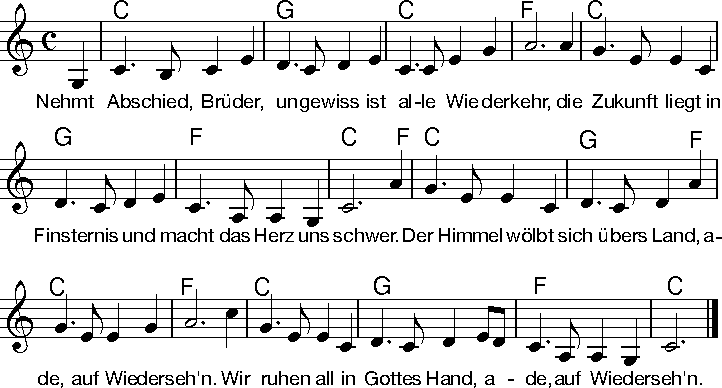
\includegraphics[width=1\textwidth]{Noten/Lied071.pdf}	

\beginverse
Die \[C]Sonne sinkt, es \[G]steigt die Nacht, ver\[C]gangen ist der \[F]Tag.
Die \[C]Welt schläft ein und \[G]leis' erwacht der \[F]Nachtigallen \[C]Schlag.
\endverse

\beginchorus
\[F]Der \[C]Himmel wölbt sich \[G]über's Land. \[F]A\[C]de, auf Wieder\[F]seh'n!
Wir \[C]ruhen all in \[G]Gottes Hand. Lebt \[F]wohl, auf Wieder\[C]seh'n! 
\endchorus

\beginverse
So ^ist in jedem ^Anbeginn das ^Ende nicht mehr ^weit.
Wir ^kommen her und ^gehen hin und ^mit uns geht die ^Zeit.
\endverse

\renewcommand{\everychorus}{\textnote{\bf Refrain (wdh.)}}
\beginchorus
\endchorus

\beginverse
Nehmt ^Abschied Brüder, ^schließt den Kreis; das ^Leben ist ein ^Spiel.
Nur ^wer es recht zu ^leben weiß, ge^langt ans große ^Ziel.
\endverse

\beginchorus
\endchorus

\endsong

\beginscripture{}
Auld Lang Syne ist der Titel eines der bekanntesten Lieder im englischsprachigen Raum. Sinngemäß bedeutet der Titel soviel wie 'längst vergangene Zeit'. Es wird in der anglophonen Welt traditionsgemäß zum Jahreswechsel gesungen, um der Verstorbenen des zu Ende gegangenen Jahres zu gedenken. Der deutsche Titel lautet „Nehmt Abschied, Brüder“. In der Pfadfinderbewegung gilt es weltweit als Abschiedslied, das am Ende von Veranstaltungen gesungen wird.

Wegen der Verwendung in der Pfadfinderbewegung wurde das Lied in zahlreiche Sprachen übertragen. Die deutsche Übertragung „Nehmt Abschied, Brüder“ von Claus Ludwig Laue entstand für die Deutsche Pfadfinderschaft Sankt Georg.
\endscripture

\begin{intersong}
\ifthenelse{\boolean{pics}}{
    \ThisLRCornerWallPaper{1}{Bilder/nehmtabschied_mikesch.jpg}
}{}
\end{intersong}